\subsection{Implementation of Polygon Guarding Algorithms for Art Gallery Problems \cite{maleki2022implementation}}
This paper \cite{maleki2022implementation} introduces implementations and their experimental evaluations for two existing approximation algorithms (\cite{GHOSH2010718}, \cite{bhattacharya2016approximability}) and a newly developed one for computing visibility in polygons in the context of the Art Gallery Problem \cite{o1987art}.

Visibility in simple planar polygons can be defined as: given a polygon $\mathcal P \subset \mathbb R^2$, a point (guard) $p \in \mathcal P$ \textit{sees} a point $q \in \mathcal P$ if the line segment $\overline{pq} \subseteq \mathcal P$. Thus, the points that are visible from $p$ form the visibility polygon (region) $\mathcal V(p)$. We distinguish between vertex guards (guards that can be placed on the vertices of $\mathcal P$) and point guards (guards that can be placed without restriction inside $\mathcal P$). If $\forall q \in \mathcal P$ is visible from some point of an edge, then $\mathcal P$ is a weak visibility polygon. All guards $p$ that can see the entirety of $\mathcal P$ form guard set $S$.

Given that computing a minimum number of guards for guarding a polygon is NP-hard \cite{1057165}, the paper will inspect how the Art Gallery Problem \cite{o1987art} can be tackled using 3 approximation algorithms.

\subsubsection{Algorithm of Ghosh \cite{GHOSH2010718}}
The algorithm of Ghosh \cite{GHOSH2010718} runs in $O(n^4)$ time and yields a $O(\log n)$-approximation for computing the minimum vertex guard for simple polygons. It begins by drawing lines through every pair of vertices of $P$ and computing the set of all its convex components $C$. It continues by constructing the sets $F_j$ through the addition of the convex components from $C$ that are totally visible from vertex $j$. Then, the algorithm recursively eliminates the redundant sets $F$ from $C$ as follows: $\forall$ fixed $j$, another vertex $i$ is searched for such that the set $F_i$ is also visible from $j$ ($|F_j| \leq |F_i|$); $F_i$ is eliminated from $C$, $i$ is added to $S$ and the process continues until $C$ is empty. At the end, $S$ contains the approximated guardset for $\mathcal P$.

\subsubsection{Algorithm of Bhattacharya \cite{bhattacharya2016approximability}}
The algorithm of Bhattacharya \cite{bhattacharya2016approximability} runs in $O(n^2)$ time and yields a 6-approximation for computing the minimum vertex guard for weak visibility polygons without holes. It begins by computing the Shortest Path Tree for the parents $u, v$ of every vertex in $\mathcal P$ and initialising all vertices as unmarked. In clockwise order from the boundary of $\mathcal P$ determined by $u, v$, every vertex $z$ is checked for visibility from $u, v$. If $\forall z$ are visible, then $u, v$ are added to $S$. Otherwise, $z$ is added to $S$ and the procedure continues with $z$ as the starting node. All vertices that become seen from $S$ are marked. At the end, the the algorithm checks whether the vertices in $S$ have overlapping visibility regions, and duplicates are removed.

\subsubsection{New Algorithm}
The algorithm introduced in the paper is focussed on polygons with large number of vertices $n$ and different amounts of reflex vertices $r$. If the number of reflex vertices is significantly lower than the total number of vertices ($r \leq \log \log n$), guards are placed at all reflex vertices. Otherwise, they are placed according to the algorithm of Ghosh \cite{GHOSH2010718}.

\subsubsection{Experiments}
Algorithms of Ghosh \cite{GHOSH2010718} and Bhattacharya \cite{bhattacharya2016approximability} are tested on weak visibility polygons, and the newly introduced algorithm is tested on simple polygons. 

Firstly, a procedure for generating arbitrary weak visibility polygons is devised: given two points $p = (k, 0), q = (-k, 0)$,  $n$ random points $x_1, ..., x_n$ sorted on the distance from $p$ on $\overline{pq}$, and $n$ sorted random angles $\alpha_1, ..., \alpha_n \in  (0, \pi)$, create $n$ vertices $y_1, ..., y_n$ by shooting $n$ rays at angle $\alpha_i, \forall x_i$. Then, add $n$ reflex vertices $z_1, ..., z_n$ as points in a quadrilateral formed by vertices $x_iy_iy_{i + 1}x_{i + 1}$. An example for such a polygon can be found in Figure \ref{fig:weak}.

\begin{figure}[h!]
    \centering
    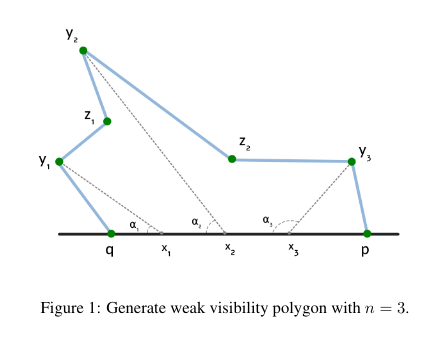
\includegraphics[width=0.6\textwidth]{Screenshot from 2022-01-24 15-07-12.png}
    \caption{}
    \label{fig:weak}
\end{figure}

The algorithms of Ghosh \cite{GHOSH2010718} and Bhattacharya \cite{bhattacharya2016approximability} were tested using arbitrarily generated polygons with $n = \overline{10, 15}$ vertices and $r \in {2, 3}$ reflex vertices. The results suggest that for low values of $n$ and $r$, the algorithm of Ghosh \cite{GHOSH2010718} performs better when using the number of guards as evaluation criteria. Its constant time approximation in this small case contrasts in this way with the constant approximation of the algorithm of Bhattacharya \cite{bhattacharya2016approximability}. Similarly, the algorithm of Ghosh \cite{GHOSH2010718} performed better both when tested on a weak visibility polygon with low $n = \overline{10, 15}$ and $\frac n 2 \leq r$, and with large $n \in \{100, 400\}$.

Secondly, a procedure for generating arbitrary simple polygons with custom number of reflex vertices $r$ is devised: starting from a simple convex polygon $\mathcal P$ with $n$ vertices, $\mathcal P$ is triangulated such that every triangle has a joint edge with its boundaries; $r$ reflex vertices are randomly added inside $\mathcal P$, and the boundaries outside of the reflex vertices are moved such that all $r$ points are now forming boundaries.

The new algorithm is tested on simple polygons constructed as previously mentioned by starting from low $r$ and gradually increase it. The results are reported positively in the sense that the $|S|$ always remains close to the optimal, as a 2-approximation solution.

Therefore, through the newly implemented algorithm, this paper \cite{maleki2022implementation} testifies that the algorithm of Ghosh \cite{GHOSH2010718} performs like a constant approximation in practice, and often better than its bound when tested on complex simple polygons.
% - guards placed on vertices = vertex guards
% - no restrictions = point guards
% - $\mathcal P$ is called weak visibility polygon if every point in $\mathcal P$ is visible from some point of an edge
% - the problem of computing a min number of guards is NP-hard
% - $O(n^4)$ approximation algorithm for computing $S$ (1)
% - $O(n^2)$ 6-approximation algorithm for vertex guarding a weak vibisility $\mathcal P$ with no holes (2)
% - implementation of algorithms and testing on weak visibility polygons
% - generating arbitrary weak visibility polygons *add algorithm* and testing them with $n = \overline{10, 15}$ and $r \in \{2, 3\}$ reflex vertices
	% - for low value of $n$ and $r$, it is better to use Algorithm 1 for minimising the number of vertex guards; since algorithm 2 is a constant approximation algorithm, algorithm 1 performs like a constant time approximation algorithm for small values of $n$ and $r$ experimentally
	% - since the criteria of minimisation is the number of guards rather than the running time which is a one-time affair unlike online algorithms, algorithm 1 is preferable even for weak visibility polygons
% - generating arbitrary weak visibility polygons and testing them with $n = \overline{10, 15}$ and $r$ reflex vertices close to the number of convex vertices
	% - for a low value of $n$ and $\frac n 2 \leq r$, algorithm 1 is better for guarding a weak visibility polygon with a min number of guards, because when the number of reflex vertices increases, the number of the diameter of the polygon and convex components decrease
% - generating arbitrary weak visibility polygons and testing them with large $n$
	% - algorithm 1 is better for guarding a weak visibility polygon with min number of guards, because it uses less guards than algorithm 2
% - generating arbitrary simply polygons *add algorithm* (Ghosh)
% - if $r << n$ , then the size of the optimal guard set is $\approx r$  => the number of edges $E$ in the visibility graph of such simple polygons is $O(n^2)$ => choose a small number $\log \log n$ as an upper bound for $r$ so that $r$ and optimal are close
% - if $r - c \leq \log \log n$, $c$ - small constant, then we place guards at all reflex vertices for guarding a simple polygon $P$, otherwise we place guards using the method of algorithm 1
% - even if $E$ reduces, the chosen guard sets remains close to the optimal and the algorithm assigns no more than twice the optimal number of guards
% => Ghosh's idea works better in practice and performs like a constant approximation algorithm